\chapter{DESARROLLO DEL PROYECTO}

\section{Descripción general del sistema}

En este capítulo se describe el desarrollo del sistema propuesto para el monitoreo de contenedores municipales en la manzana del Mercado San Camilo, Arequipa. El sistema está conformado por nodos IoT instalados en los contenedores, una red de comunicación LoRa P2P, un gateway LoRa-WiFi, un servidor central y una plataforma de monitoreo.

El objetivo de este capítulo es presentar el proceso de diseño, selección de componentes, construcción del prototipo, configuración de red, desarrollo del software e integración del sistema. Los resultados obtenidos durante las pruebas y su análisis serán presentados en el capítulo correspondiente a resultados y discusión.

\section{Selección e implementación de componentes}
El sistema está conformado por dos bloques principales de hardware: el nodo IoT y el gateway LoRa-P2P.El nodo IoT se encarga de medir el estado del contenedor municipal y transmitir los datos mediante comunicación LoRa P2P. Por otro lado, el gateway recibe los paquetes enviados por los nodos, registra métricas de comunicación y reenvía la información hacia el servidor central mediante MQTT. Los componentes principales del sistema se resumen en la abla~\ref{tab:componentes_nodo_gateway}.

\subsection{Componentes del nodo IoT}

El nodo IoT es el dispositivo encargado de medir el estado del contenedor municipal y transmitir los datos hacia el gateway mediante comunicación LoRa P2P. Para su implementación se consideran los siguientes componentes principales:

\begin{itemize}
    \item Microcontrolador ESP32 Dev Kit.
    \item Módulo LoRa SX1278.
    \item Sensor de nivel de llenado.
    \item Sensor de temperatura y humedad.
    \item Sensor de gases o calidad de aire.
    \item Sensor de batería o medición de voltaje.
    \item Antena LoRa.
    \item Sistema de alimentación.
    \item Caja de protección para instalación en campo.
\end{itemize}

\subsection{Componentes del gateway LoRa-WiFi}

El gateway LoRa-WiFi cumple la función de recibir los paquetes transmitidos por los nodos y reenviarlos hacia el servidor central. Para su implementación se consideran los siguientes componentes:

\begin{itemize}
    \item Microcontrolador ESP32-S3.
    \item Módulo LoRa SX1278.
    \item Antena LoRa.
    \item Pantalla OLED para visualización local.
    \item Conectividad WiFi.
    \item Fuente de alimentación.
    \item Caja de protección para el gateway.
\end{itemize}
\begingroup
\small
\renewcommand{\arraystretch}{1.2}
\begin{xltabular}{\linewidth}{
>{\raggedright\arraybackslash}p{2.4cm}
>{\raggedright\arraybackslash}p{3.2cm}
>{\raggedright\arraybackslash}p{3.6cm}
>{\raggedright\arraybackslash}X}
\caption{Componentes principales del nodo IoT y gateway LoRa-WiFi.}
\label{tab:componentes_nodo_gateway} \\
\toprule
\textbf{Bloque} & \textbf{Componente} & \textbf{Función} & \textbf{Justificación de uso} \\
\midrule
\endfirsthead

\multicolumn{4}{c}{\tablename\ \thetable{} -- Continúa de la página anterior} \\
\toprule
\textbf{Bloque} & \textbf{Componente} & \textbf{Función} & \textbf{Justificación de uso} \\
\midrule
\endhead

\midrule
\multicolumn{4}{r}{\textit{Continúa en la siguiente página...}} \\
\endfoot

\bottomrule
\endlastfoot

\textbf{Nodo IoT} 
& ESP32 Dev Kit V1 
& Unidad de procesamiento del nodo 
& Permite adquirir datos de sensores, procesar la información y controlar la transmisión mediante LoRa P2P. \\

\textbf{Nodo IoT} 
& Módulo LoRa SX1278 
& Comunicación inalámbrica 
& Permite transmitir los datos del contenedor hacia el gateway mediante comunicación LoRa P2P de largo alcance. \\

\textbf{Nodo IoT} 
& Sensor VL53L1X 
& Medición del nivel de llenado 
& Permite estimar la distancia entre el sensor y los residuos, ayudando a determinar el estado de llenado del contenedor. \\

\textbf{Nodo IoT} 
& Sensor ultrasónico HC-SR04 
& Medición complementaria de distancia 
& Puede utilizarse como apoyo para validar o comparar la medición del nivel de llenado. \\

\textbf{Nodo IoT} 
& Sensor DHT11 
& Medición de temperatura y humedad 
& Permite registrar condiciones ambientales relacionadas con el entorno del contenedor. \\

\textbf{Nodo IoT} 
& Sensor MQ135 
& Detección de gases o calidad de aire 
& Permite identificar variaciones asociadas a malos olores o acumulación de residuos. \\

\textbf{Nodo IoT} 
& Sensor infrarrojo HW-201 
& Detección de presencia u obstáculo 
& Apoya la detección de objetos o residuos dentro del rango de medición del sistema. \\

\textbf{Nodo IoT} 
& Módulo GPS NEO-6M 
& Ubicación del nodo 
& Permite registrar la posición del contenedor; su uso puede ser opcional si la ubicación del contenedor es fija. \\

\textbf{Nodo IoT} 
& Sistema de alimentación 
& Energía del nodo 
& Proporciona la energía necesaria para el funcionamiento del ESP32, sensores y módulo LoRa. \\

\textbf{Nodo IoT} 
& Antena LoRa 
& Mejora de transmisión 
& Permite mejorar el enlace inalámbrico entre el nodo y el gateway. \\

\textbf{Nodo IoT} 
& Caja de protección 
& Protección física 
& Protege los componentes electrónicos frente a polvo, humedad, golpes o manipulación externa. \\

\midrule

\textbf{Gateway} 
& ESP32-S3 Dev Kit 
& Unidad principal del gateway 
& Permite recibir, procesar y reenviar los datos hacia el servidor central. Se selecciona por su mayor capacidad de procesamiento frente al ESP32 básico. \\

\textbf{Gateway} 
& Módulo LoRa SX1278 
& Recepción de paquetes LoRa 
& Permite recibir los paquetes transmitidos por los nodos IoT mediante comunicación LoRa P2P. \\

\textbf{Gateway} 
& Antena LoRa 
& Mejora de recepción 
& Mejora la recepción de paquetes enviados por los nodos y contribuye a la estabilidad del enlace inalámbrico. \\

\textbf{Gateway} 
& Pantalla OLED 0.96'' I2C 
& Visualización local 
& Permite mostrar información básica del gateway, como estado de conexión, paquetes recibidos, RSSI, SNR o identificador del nodo. \\

\textbf{Gateway} 
& Conectividad WiFi 
& Envío de datos al servidor 
& Permite conectar el gateway con el servidor central para publicar la información mediante MQTT. \\

\textbf{Gateway} 
& Fuente de alimentación 
& Energía del gateway 
& Proporciona alimentación continua al gateway, debido a que debe mantenerse activo para recibir paquetes de los nodos. \\

\textbf{Gateway} 
& Caja de protección 
& Protección física 
& Protege el gateway frente a polvo, humedad, golpes o condiciones del entorno durante las pruebas. \\

\bottomrule
\end{xltabular}
\endgroup

\subsection{Componentes de la plataforma y servidor}

La plataforma de monitoreo permite visualizar el estado de los contenedores, nodos, gateway y métricas de red. Para su implementación se emplean los siguientes servicios y herramientas:

\begin{itemize}
    \item React para el desarrollo del frontend.
    \item Fastify para el desarrollo de la API backend.
    \item Mosquitto como broker MQTT.
    \item PostgreSQL para almacenamiento de datos estructurados.
    \item InfluxDB para almacenamiento de telemetría y métricas temporales.
    \item Docker para el despliegue de servicios.
    \item Servidor VPS para alojar la plataforma.
\end{itemize}

\section{Diseño de la red y arquitectura del sistema}

En esta sección se describe la arquitectura general del sistema y la forma en que se comunican los distintos componentes. La arquitectura propuesta integra nodos IoT, comunicación LoRa P2P, gateway LoRa-WiFi, servidor central y plataforma de monitoreo.

\subsection{Diagrama de bloques}

El diagrama de bloques representa la estructura general del sistema y la relación entre sus principales componentes. El sistema está conformado por los nodos de monitoreo, el gateway LoRa-WiFi, los servicios del servidor, las bases de datos y la plataforma web.

\begin{figure}[H]
    \centering
    \resizebox{0.96\textwidth}{!}{
    \begin{tikzpicture}[
        node distance=1.8cm,
        bloque/.style={
            rectangle,
            rounded corners=3pt,
            draw=black,
            line width=0.8pt,
            align=center,
            text width=3.3cm,
            minimum width=3.7cm,
            minimum height=3cm,
            inner sep=5pt,
            fill=blue!7
        },
        flecha/.style={
            -{Latex[length=3mm,width=2mm]},
            line width=0.8pt
        },
        textoFlecha/.style={
            font=\scriptsize,
            align=center,
            text width=1.7cm,
            inner sep=0pt
        }
    ]

    \node[bloque] (nodos) {
        \textbf{Nodos IoT}\\[2mm]
        ESP32 Dev Kit\\
        Sensores del contenedor\\
        Módulo LoRa SX1278\\
        Alimentación por batería
    };

    \node[bloque, right=of nodos] (gateway) {
        \textbf{Gateway LoRa-WiFi}\\[2mm]
        ESP32-S3\\
        Módulo LoRa SX1278\\
        Registro de RSSI y SNR\\
        Conectividad WiFi
    };

    \node[bloque, right=of gateway] (servicios) {
        \textbf{Servicios del servidor}\\[2mm]
        Mosquitto MQTT\\
        API Fastify\\
        Procesamiento de datos\\
        Contenedores Docker
    };

    \node[bloque, right=of servicios] (datos) {
        \textbf{Bases de datos}\\[2mm]
        PostgreSQL\\
        InfluxDB\\
        Datos estructurados\\
        Series temporales
    };

    \node[bloque, right=of datos] (plataforma) {
        \textbf{Plataforma web}\\[2mm]
        Frontend React\\
        Estado de contenedores\\
        Alertas e históricos\\
        Métricas de red
    };

    \draw[flecha] (nodos) -- 
        node[midway, above=2pt, textoFlecha] {LoRa P2P}
        (gateway);

    \draw[flecha] (gateway) -- 
        node[midway, above=2pt, textoFlecha] {MQTT}
        (servicios);

    \draw[flecha] (servicios) -- 
        node[midway, above=2pt, textoFlecha] {Consultas}
        (datos);

    \draw[flecha] (datos) -- 
        node[midway, above=2pt, textoFlecha] {API REST}
        (plataforma);

    \end{tikzpicture}
    }

    \caption{Diagrama de bloques de la arquitectura general del sistema.}
    \label{fig:diagrama_bloques_sistema}
\end{figure}

El flujo inicia en los nodos IoT, donde se adquieren los datos del contenedor. La información se transmite mediante LoRa P2P hacia el gateway, que posteriormente la publica mediante MQTT hacia el servidor. Los datos son procesados y almacenados en PostgreSQL e InfluxDB para su consulta y visualización en la plataforma web.

\subsection{Diagrama de flujo}

El diagrama de flujo describe la secuencia de funcionamiento del sistema, desde la adquisición de datos en el nodo IoT hasta su almacenamiento y visualización en la plataforma web. La Figura~\ref{fig:flujo_funcionamiento_sistema} muestra las etapas de medición, transmisión, recepción, procesamiento y generación de alertas.

\begin{figure}[H]
    \centering
    \resizebox{0.48\textwidth}{!}{
    \begin{tikzpicture}[
        node distance=0.65cm,
        proceso/.style={
            rectangle,
            rounded corners=3pt,
            draw=black,
            line width=0.8pt,
            align=center,
            text width=5.2cm,
            minimum height=0.85cm,
            fill=blue!7
        },
        decision/.style={
            diamond,
            draw=black,
            line width=0.8pt,
            align=center,
            text width=3.2cm,
            aspect=2.2,
            inner sep=1pt,
            fill=yellow!12
        },
        iniciofin/.style={
            ellipse,
            draw=black,
            line width=0.8pt,
            align=center,
            text width=3.7cm,
            minimum height=0.8cm,
            fill=green!10
        },
        flecha/.style={
            -{Latex[length=2.5mm]},
            line width=0.8pt
        },
        texto/.style={
            font=\scriptsize
        }
    ]

    \node[iniciofin] (inicio) {
        \textbf{Inicio del ciclo}
    };

    \node[proceso, below=of inicio] (lectura) {
        \textbf{Lectura de sensores}\\
        Nivel de llenado, temperatura, humedad, gases y batería
    };

    \node[proceso, below=of lectura] (procesamiento) {
        \textbf{Procesamiento en el nodo IoT}\\
        Validación y conversión de las mediciones
    };

    \node[decision, below=of procesamiento] (datosvalidos) {
        ¿Datos válidos?
    };

    \node[proceso, right=1.8cm of datosvalidos] (relectura) {
        Repetir lectura y verificar sensores
    };

    \node[proceso, below=of datosvalidos] (paquete) {
        \textbf{Construcción del paquete}\\
        ID de nodo, número de paquete, mediciones y estado
    };

    \node[proceso, below=of paquete] (transmision) {
        \textbf{Transmisión LoRa P2P}\\
        Envío del paquete hacia el gateway
    };

    \node[proceso, below=of transmision] (gateway) {
        \textbf{Recepción en el gateway}\\
        Validación del paquete y registro de RSSI y SNR
    };

    \node[decision, below=of gateway] (wifi) {
        ¿Conexión WiFi disponible?
    };

    \node[proceso, right=1.8cm of wifi] (espera) {
        Almacenar temporalmente y reintentar conexión
    };

    \node[proceso, below=of wifi] (mqtt) {
        \textbf{Publicación mediante MQTT}\\
        Envío de la telemetría hacia el servidor central
    };

    \node[proceso, below=of mqtt] (almacenamiento) {
        \textbf{Procesamiento y almacenamiento}\\
        API Fastify, PostgreSQL e InfluxDB
    };

    \node[decision, below=of almacenamiento] (critico) {
        ¿Estado crítico?
    };

    \node[proceso, right=1.8cm of critico] (alerta) {
        Generar alerta de llenado, gases o batería baja
    };

    \node[proceso, below=of critico] (visualizacion) {
        \textbf{Visualización en la plataforma}\\
        Contenedores, métricas de red, históricos y alertas
    };

    \node[iniciofin, below=of visualizacion] (esperaciclo) {
        Esperar el siguiente intervalo de medición
    };

    \draw[flecha] (inicio) -- (lectura);
    \draw[flecha] (lectura) -- (procesamiento);
    \draw[flecha] (procesamiento) -- (datosvalidos);

    \draw[flecha] (datosvalidos) --
        node[right, texto]{Sí}
        (paquete);

    \draw[flecha] (datosvalidos) --
        node[above, texto]{No}
        (relectura);

    \draw[flecha] (relectura) |- (lectura);

    \draw[flecha] (paquete) -- (transmision);
    \draw[flecha] (transmision) -- (gateway);
    \draw[flecha] (gateway) -- (wifi);

    \draw[flecha] (wifi) --
        node[right, texto]{Sí}
        (mqtt);

    \draw[flecha] (wifi) --
        node[above, texto]{No}
        (espera);

    \draw[flecha] (espera) |- (wifi);

    \draw[flecha] (mqtt) -- (almacenamiento);
    \draw[flecha] (almacenamiento) -- (critico);

    \draw[flecha] (critico) --
        node[right, texto]{No}
        (visualizacion);

    \draw[flecha] (critico) --
        node[above, texto]{Sí}
        (alerta);

    \draw[flecha] (alerta) |- (visualizacion);
    \draw[flecha] (visualizacion) -- (esperaciclo);
    \draw[flecha] (esperaciclo.west) -- ++(-1.2,0) |- (lectura.west);

    \end{tikzpicture}
    }

    \caption{Diagrama de flujo del funcionamiento general del sistema.}
    \label{fig:flujo_funcionamiento_sistema}
\end{figure}

El flujo comienza con la lectura de los sensores instalados en el contenedor. El nodo valida las mediciones, construye un paquete de datos y lo transmite mediante LoRa P2P hacia el gateway. Este registra las métricas RSSI y SNR y publica la información mediante MQTT cuando dispone de conexión WiFi.

Posteriormente, el servidor procesa y almacena los datos en PostgreSQL e InfluxDB. Si se detecta un nivel crítico de llenado, presencia elevada de gases o batería baja, el sistema genera una alerta. Finalmente, la información se presenta en la plataforma web y el nodo espera el siguiente intervalo para repetir el ciclo.


\subsection{Arquitectura de comunicación LoRa P2P}

La arquitectura de comunicación propuesta utiliza una topología tipo estrella, en la cual varios nodos IoT transmiten directamente hacia un gateway LoRa-WiFi mediante enlaces LoRa P2P. Cada nodo dispone de un identificador único y genera paquetes que contienen las mediciones del contenedor, el número secuencial del paquete y el estado energético del dispositivo.
Todos los nodos deben utilizar parámetros de radio compatibles, como frecuencia de operación, ancho de banda, factor de dispersión, tasa de codificación y potencia de transmisión. El gateway permanece en modo recepción, identifica el origen de cada paquete y registra métricas como RSSI y SNR. Posteriormente, la información es reenviada hacia el servidor central mediante MQTT.
\begin{figure}[H]
    \centering
    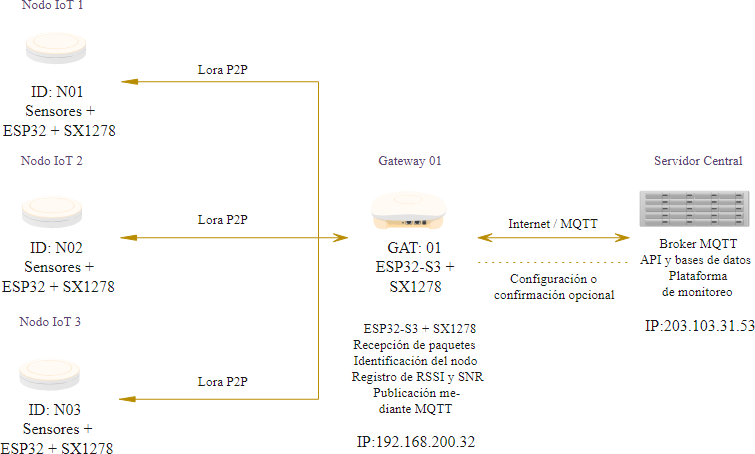
\includegraphics[width=0.85\textwidth]{figures/red.pdf}
    \caption{Diseño de la red de comunicación del sistema.}
    \label{fig:diseno_red}
\end{figure}

La comunicación se realiza principalmente en sentido ascendente, desde los nodos hacia el gateway. Para diferenciar las transmisiones, cada paquete incorpora un identificador de nodo y un número secuencial. Estos campos permiten detectar paquetes duplicados, estimar pérdidas y calcular métricas como PDR y PLR.

Con el fin de reducir transmisiones simultáneas, la arquitectura puede incorporar intervalos diferenciados, retardos aleatorios y transmisión por eventos. Las confirmaciones o mensajes descendentes deben utilizarse únicamente cuando sean necesarios, debido a que incrementan el tiempo en aire y el consumo energético.

\begin{table}[H]
\centering
\caption{Características de la arquitectura LoRa P2P propuesta.}
\label{tab:arquitectura_lora_p2p}
\small
\renewcommand{\arraystretch}{1.2}
\begin{tabularx}{\linewidth}{
>{\raggedright\arraybackslash}p{4.2cm}
>{\raggedright\arraybackslash}X}
\toprule
\textbf{Característica} & \textbf{Descripción} \\
\midrule
Topología & Estrella, con varios nodos asociados a un gateway. \\
Modo de comunicación & LoRa punto a punto, sin servidor de red LoRaWAN. \\
Identificación & Identificador único de nodo y número secuencial de paquete. \\
Parámetros compartidos & Frecuencia, ancho de banda, factor de dispersión, tasa de codificación y potencia de transmisión. \\
Métricas registradas & RSSI, SNR, paquetes enviados, paquetes recibidos, PDR, PLR y latencia. \\
Control de acceso & Intervalos de transmisión, retardo aleatorio y transmisión por evento. \\
Salida del gateway & Publicación de telemetría hacia el servidor mediante MQTT. \\
\bottomrule
\end{tabularx}
\end{table}

La comunicación entre los nodos y el gateway se realiza mediante LoRa P2P. En este esquema, cada nodo transmite paquetes de datos hacia un gateway propio, sin utilizar una infraestructura LoRaWAN.

Para esta arquitectura se consideran los siguientes elementos:

\begin{itemize}
    \item Identificador único de nodo.
    \item Número incremental de paquete.
    \item Formato compacto de datos.
    \item Parámetros de comunicación LoRa.
    \item Control de intervalos de transmisión.
    \item Registro de RSSI y SNR en el gateway.
\end{itemize}

\subsection{Flujo de datos del sistema}

El flujo de datos del sistema comienza con la adquisición de las variables físicas del contenedor y finaliza con su almacenamiento y visualización en la plataforma web. Durante este proceso, la información es validada, empaquetada, transmitida, procesada y registrada junto con las métricas de comunicación obtenidas por el gateway.El proceso comienza con la lectura de los sensores instalados en el contenedor. El ESP32 valida y procesa las mediciones antes de construir un paquete compacto que incluye el identificador del nodo, el número secuencial, las variables medidas y el estado energético.

El paquete se transmite mediante LoRa P2P hacia el gateway. Al recibirlo, el gateway incorpora información adicional del enlace, como RSSI, SNR y la marca temporal, y posteriormente publica la telemetría mediante MQTT hacia el servidor central.
La Figura~\ref{fig:flujo_datos_sistema} presenta el recorrido de la información entre los diferentes componentes del sistema.En el servidor, la API desarrollada con Fastify valida y clasifica la información. Los datos estructurados, como nodos, contenedores y configuración, se almacenan en PostgreSQL, mientras que las mediciones y métricas temporales se registran en InfluxDB. Finalmente, la plataforma desarrollada en React consulta estos datos para mostrar el estado de los contenedores, alertas, históricos y métricas de la red LoRa P2P.
\begin{figure}[H]
    \centering
    \resizebox{0.28\textwidth}{!}{
    \begin{tikzpicture}[
        node distance=0.75cm,
        bloque/.style={
            rectangle,
            rounded corners=3pt,
            draw=black,
            line width=0.8pt,
            align=center,
            text width=6.0cm,
            minimum height=1.05cm,
            inner sep=5pt,
            fill=blue!7
        },
        almacenamiento/.style={
            rectangle,
            rounded corners=3pt,
            draw=black,
            line width=0.8pt,
            align=center,
            text width=6.0cm,
            minimum height=1.05cm,
            inner sep=5pt,
            fill=green!9
        },
        interfaz/.style={
            rectangle,
            rounded corners=3pt,
            draw=black,
            line width=0.8pt,
            align=center,
            text width=6.0cm,
            minimum height=1.05cm,
            inner sep=5pt,
            fill=violet!8
        },
        flecha/.style={
            -{Latex[length=2.6mm,width=1.8mm]},
            line width=0.8pt
        },
        etiqueta/.style={
            font=\scriptsize,
            fill=white,
            inner sep=1pt
        }
    ]

    \node[bloque] (sensores) {
        \textbf{1. Adquisición de datos}\\
        Nivel de llenado, temperatura, humedad, gases y batería
    };

    \node[bloque, below=of sensores] (nodo) {
        \textbf{2. Procesamiento en el nodo IoT}\\
        Validación, conversión de mediciones y determinación del estado del contenedor
    };

    \node[bloque, below=of nodo] (paquete) {
        \textbf{3. Construcción del paquete LoRa}\\
        ID del nodo, número de paquete, mediciones, batería y estado
    };

    \node[bloque, below=of paquete] (lora) {
        \textbf{4. Transmisión LoRa P2P}\\
        Envío inalámbrico del paquete hacia el gateway
    };

    \node[bloque, below=of lora] (gateway) {
        \textbf{5. Procesamiento en el gateway}\\
        Validación del paquete, registro de RSSI, SNR y marca temporal
    };

    \node[bloque, below=of gateway] (mqtt) {
        \textbf{6. Publicación mediante MQTT}\\
        Envío de telemetría hacia el broker Mosquitto del servidor central
    };

    \node[bloque, below=of mqtt] (backend) {
        \textbf{7. Procesamiento en el backend}\\
        Validación, clasificación de datos y generación de alertas
    };

    \node[almacenamiento, below=of backend] (bases) {
        \textbf{8. Almacenamiento}\\
        PostgreSQL para datos estructurados e InfluxDB para series temporales
    };

    \node[interfaz, below=of bases] (plataforma) {
        \textbf{9. Visualización en la plataforma web}\\
        Estado de contenedores, métricas de red, alertas e históricos
    };

    \draw[flecha] (sensores.south) --
        node[right, etiqueta]{Lecturas}
        (nodo.north);

    \draw[flecha] (nodo.south) --
        node[right, etiqueta]{Datos procesados}
        (paquete.north);

    \draw[flecha] (paquete.south) --
        node[right, etiqueta]{Payload}
        (lora.north);

    \draw[flecha] (lora.south) --
        node[right, etiqueta]{Paquete LoRa}
        (gateway.north);

    \draw[flecha] (gateway.south) --
        node[right, etiqueta]{Telemetría enriquecida}
        (mqtt.north);

    \draw[flecha] (mqtt.south) --
        node[right, etiqueta]{Mensaje MQTT}
        (backend.north);

    \draw[flecha] (backend.south) --
        node[right, etiqueta]{Datos validados}
        (bases.north);

    \draw[flecha] (bases.south) --
        node[right, etiqueta]{Consultas}
        (plataforma.north);

    \end{tikzpicture}
    }

    \caption{Flujo de datos del sistema de monitoreo.}
    \label{fig:flujo_datos_sistema}
\end{figure}

\begin{table}[H]
\centering
\caption{Datos procesados en cada etapa del sistema.}
\label{tab:flujo_datos_sistema}
\small
\renewcommand{\arraystretch}{1.2}
\begin{tabularx}{\linewidth}{
>{\raggedright\arraybackslash}p{3.5cm}
>{\raggedright\arraybackslash}X
>{\raggedright\arraybackslash}p{3.6cm}}
\toprule
\textbf{Etapa} & \textbf{Datos procesados} & \textbf{Destino} \\
\midrule
Sensores
& Nivel de llenado, temperatura, humedad, gases y batería.
& ESP32 del nodo. \\

Nodo IoT
& Datos validados, ID de nodo, número de paquete y estado del contenedor.
& Módulo LoRa SX1278. \\

Comunicación LoRa P2P
& Paquete compacto de telemetría.
& Gateway LoRa-WiFi. \\

Gateway
& Telemetría, RSSI, SNR y marca temporal.
& Broker MQTT. \\

Backend
& Datos validados, eventos y alertas.
& PostgreSQL e InfluxDB. \\

Plataforma web
& Estado actual, históricos y métricas de comunicación.
& Usuario del sistema. \\
\bottomrule
\end{tabularx}
\end{table}
\section{Prototipado del sistema}

En esta sección se describe la construcción física del prototipo, incluyendo el montaje del nodo IoT, el montaje del gateway y la configuración inicial de los dispositivos.

\subsection{Montaje del nodo IoT}

El montaje del nodo IoT comprende la conexión del microcontrolador ESP32 con el módulo LoRa SX1278 y los sensores seleccionados. Cada sensor se conecta a los pines correspondientes del ESP32 según su tipo de señal, ya sea digital, analógica, I2C o UART.

El nodo debe ser instalado dentro de una caja de protección para reducir el riesgo de daño por polvo, humedad, golpes o manipulación externa. Además, se debe considerar una ubicación adecuada dentro o cerca del contenedor para permitir una correcta medición del nivel de llenado.

\subsection{Montaje del gateway LoRa-WiFi}

El gateway se implementa utilizando un ESP32-S3, un módulo LoRa SX1278 y una pantalla OLED. El módulo LoRa se encarga de recibir los paquetes enviados por los nodos, mientras que el ESP32-S3 procesa la información y la publica hacia el servidor mediante MQTT.

La pantalla OLED permite mostrar información básica del estado del gateway, como conexión WiFi, paquetes recibidos, identificador del nodo y métricas de comunicación.

\subsection{Configuración de sensores y módulo LoRa}

La configuración de sensores incluye la lectura de las variables del contenedor, tales como nivel de llenado, temperatura, humedad, gases y batería. Estas mediciones son procesadas por el microcontrolador antes de ser enviadas hacia el gateway.

La configuración del módulo LoRa comprende la definición de parámetros como frecuencia de operación, potencia de transmisión, ancho de banda, factor de dispersión y formato del paquete.

\subsection{Configuración de red y conectividad}

En esta etapa se configura la comunicación entre el gateway y el servidor central. El gateway se conecta a una red WiFi disponible y publica los datos recibidos mediante MQTT hacia el broker Mosquitto desplegado en el servidor VPS.

\section{Desarrollo del software}

En esta sección se describe el desarrollo del software necesario para el funcionamiento del sistema, incluyendo firmware, backend, broker MQTT, bases de datos y frontend.

\subsection{Firmware del nodo IoT}

El firmware del nodo IoT permite adquirir datos de los sensores, construir el paquete de información y transmitirlo mediante LoRa P2P. Además, puede incorporar lógica de transmisión adaptativa para reducir envíos innecesarios y optimizar el consumo energético.

El paquete enviado por el nodo puede incluir:

\begin{itemize}
    \item Identificador del nodo.
    \item Número de paquete.
    \item Nivel de llenado.
    \item Temperatura.
    \item Humedad.
    \item Lectura de gases.
    \item Estado de batería.
    \item Estado del contenedor.
\end{itemize}

\subsection{Firmware del gateway}

El firmware del gateway permite recibir paquetes LoRa P2P, extraer los datos enviados por los nodos, registrar RSSI y SNR, validar la información recibida y publicar la telemetría hacia el servidor central mediante MQTT.

\subsection{Backend y API}

El backend se desarrolla utilizando Fastify. Su función es procesar la información recibida, gestionar consultas desde la plataforma web y administrar datos relacionados con nodos, contenedores, gateway, métricas y alertas.

\subsection{Broker MQTT}

Mosquitto se utiliza como broker MQTT para recibir la telemetría enviada por el gateway. El modelo publicador/suscriptor permite desacoplar la transmisión de datos desde el gateway y el procesamiento posterior en el servidor.

\subsection{Base de datos}

El sistema emplea dos tipos de bases de datos:

\begin{itemize}
    \item \textbf{PostgreSQL:} para almacenar datos estructurados como usuarios, nodos, contenedores, gateway, configuración y alertas.
    \item \textbf{InfluxDB:} para almacenar datos temporales como nivel de llenado, RSSI, SNR, batería, latencia y registros de telemetría.
\end{itemize}

\subsection{Frontend y plataforma de monitoreo}

El frontend se desarrolla en React y permite visualizar la información del sistema mediante una interfaz web. La plataforma puede incluir vistas para:

\begin{itemize}
    \item Estado de contenedores.
    \item Estado de nodos.
    \item Estado del gateway.
    \item Métricas de red.
    \item Alertas.
    \item Datos históricos.
\end{itemize}

\section{Integración del sistema}

La integración del sistema consiste en conectar todos los componentes desarrollados para asegurar el funcionamiento completo del flujo de datos, desde el nodo IoT hasta la plataforma web.

\subsection{Integración nodo--gateway}

En esta etapa se verifica que los nodos puedan transmitir correctamente los paquetes mediante LoRa P2P y que el gateway pueda recibirlos, identificar el nodo transmisor y registrar las métricas de comunicación.

\subsection{Integración gateway--servidor}

En esta etapa se verifica que el gateway pueda conectarse a la red WiFi y publicar los datos hacia el broker MQTT desplegado en el servidor central.

\subsection{Integración servidor--plataforma}

En esta etapa se verifica que los datos recibidos por el servidor sean almacenados correctamente en las bases de datos y puedan ser consultados desde la plataforma web.

\section{Plan de pruebas}

En esta sección se presenta el plan de pruebas definido para verificar el funcionamiento del sistema. Los resultados obtenidos serán desarrollados en el capítulo de resultados y discusión.

\subsection{Pruebas de sensores}

Se realizarán pruebas para verificar la lectura del nivel de llenado, temperatura, humedad, gases y estado de batería. Estas pruebas permitirán validar que los sensores entreguen datos coherentes para el monitoreo del contenedor.

\subsection{Pruebas de comunicación LoRa P2P}

Se realizarán pruebas de comunicación entre nodos y gateway, registrando métricas como RSSI, SNR, paquetes enviados, paquetes recibidos, pérdida de paquetes y latencia.

\subsection{Pruebas de plataforma}

Se verificará que la plataforma reciba, almacene y visualice correctamente los datos enviados desde el gateway. También se comprobará la visualización de alertas y métricas de red.

\subsection{Pruebas de funcionamiento integral}

Se validará el flujo completo del sistema, desde la adquisición de datos en el nodo IoT hasta la visualización en la plataforma web. Esta prueba permitirá comprobar la integración entre hardware, comunicación, servidor y software de monitoreo.

\begin{conceptcard}{Frecuencia de corte}
Para el modo dominante $\text{TE}_{10}$, la frecuencia de corte es el límite físico por debajo del cual no hay propagación. Se expresa como:
\begin{equation}
f_c = \frac{c}{2a}
\end{equation}
donde $c$ es la velocidad de la luz y $a$ es el ancho interno de la guía.
\end{conceptcard}

Para que exista propagación, la frecuencia de operación debe ser mayor que la frecuencia de corte. Si la frecuencia es menor, la onda no se propaga adecuadamente y se atenúa dentro de la estructura.

\section{Guía de onda WR42}

La guía WR42 es una guía rectangular empleada en aplicaciones de microondas. En esta práctica se utiliza una estructura con dimensiones internas aproximadas de $420$ mils de ancho y $170$ mils de alto, diseñada para operar alrededor de $20$ GHz.Este tipo de guía resulta adecuada para aplicaciones de alta frecuencia debido a sus bajas pérdidas, buen confinamiento del campo electromagnético y capacidad para manejar niveles elevados de potencia. Por esta razón, es utilizada en sistemas como radares, comunicaciones satelitales, enlaces de microondas y redes de combinación de potencia.

\section{Combinadores de potencia}

Un combinador de potencia es un dispositivo pasivo que permite sumar señales provenientes de dos o más entradas y dirigir la energía resultante hacia un puerto de salida. En esta práctica se analiza un combinador de cuatro puertos, donde dos puertos actúan como entradas, uno como salida combinada y otro como puerto aislado. El funcionamiento del combinador depende de la magnitud y la fase de las señales aplicadas. Cuando las señales de entrada presentan la relación de fase adecuada, la energía se combina de manera constructiva hacia el puerto de salida. Al mismo tiempo, la energía no deseada o reflejada debe dirigirse preferiblemente hacia el puerto aislado.

\section{Parámetros de dispersión}

Los parámetros de dispersión, o parámetros $S$, permiten describir el comportamiento de una red de microondas a partir de ondas incidentes y reflejadas. 
\begin{conceptcard}{Definición de $S_{ij}$}

El parámetro $S_{ij}$ representa la relación entre la onda saliente en el puerto $i$ y la onda incidente en el puerto $j$:

\begin{equation}
S_{ij}=\frac{b_i}{a_j}
\end{equation}

\end{conceptcard}

En este laboratorio, los parámetros más importantes son:

\begin{itemize}
\item $S_{11}$: indica la reflexión en el puerto de referencia. Un valor bajo en magnitud representa buena adaptación.
\item $S_{12}$ y $S_{14}$: permiten evaluar la transferencia de potencia entre los puertos principales del combinador.
\item $S_{13}$: se asocia con el aislamiento entre el puerto de salida y el puerto aislado.
\end{itemize}

Los parámetros $S$ suelen expresarse en decibelios mediante:

\begin{equation}
S_{ij}(\text{dB}) = 20\log_{10}\left|S_{ij}\right|
\end{equation}

Un valor más negativo indica menor reflexión o menor transmisión, dependiendo del parámetro analizado.

\section{Pérdida de retorno}

La pérdida de retorno permite evaluar la cantidad de energía que se refleja en un puerto debido a desadaptaciones de impedancia. Se relaciona directamente con el parámetro $S_{11}$:

\begin{equation}
\text{RL} = -20\log_{10}\left|S_{11}\right|
\end{equation}

Una pérdida de retorno alta indica que el puerto se encuentra bien adaptado, ya que una menor parte de la señal incidente es reflejada hacia la fuente.

\section{Pérdida de inserción}

La pérdida de inserción mide la reducción de potencia cuando la señal se transmite desde un puerto de entrada hacia un puerto de salida. Para una transmisión entre los puertos $j$ e $i$, se expresa como:

\begin{equation}
\text{IL} = -20\log_{10}\left|S_{ij}\right|
\end{equation}

En un combinador de potencia, la pérdida de inserción debe ser baja para que la mayor cantidad posible de energía llegue al puerto de salida. Si esta pérdida aumenta, el dispositivo entrega menos potencia útil y su eficiencia disminuye.

\section{Aislamiento}

El aislamiento indica qué tan desacoplados se encuentran dos puertos que idealmente no deberían intercambiar energía. En el caso del combinador, el puerto aislado debe recibir la menor cantidad posible de potencia durante la operación normal.Un buen aislamiento se evidencia cuando el parámetro asociado al puerto aislado presenta un valor muy negativo en decibelios. Esto significa que la señal transmitida hacia ese puerto es pequeña en comparación con la señal incidente.

\section{Wave Ports en HFSS}

Los \textit{Wave Ports} son excitaciones utilizadas en HFSS para introducir y medir ondas electromagnéticas en estructuras como guías de onda. Estos puertos permiten calcular los modos de propagación, la impedancia modal y los parámetros $S$ del sistema.La correcta asignación de los puertos es fundamental, ya que de ella depende que la simulación represente adecuadamente el comportamiento físico del dispositivo. Un puerto mal definido puede generar resultados incorrectos, modos no deseados o errores en la interpretación de la transmisión y reflexión.

\section{Condiciones de frontera en HFSS}

Las condiciones de frontera definen cómo interactúan los campos electromagnéticos con las superficies del modelo. En una guía de onda, las paredes metálicas confinan el campo y permiten la propagación de la energía dentro de la estructura.En HFSS pueden emplearse fronteras conductoras para representar las paredes metálicas del dispositivo. Si se considera una conductividad finita, el modelo toma en cuenta pérdidas asociadas al material conductor, lo cual permite obtener una simulación más cercana al comportamiento real.

\section{Simetría Perfect E}

Cuando una estructura presenta simetría geométrica y electromagnética, es posible reducir el dominio de simulación aplicando una condición de simetría. En esta práctica se utiliza una frontera tipo \textit{Perfect E}, la cual permite modelar solo una parte del combinador y representar el efecto del resto de la estructura.

El uso de esta condición reduce el número de elementos de malla y disminuye el tiempo de simulación, sin afectar la validez física del modelo cuando la simetría ha sido correctamente aplicada.

\section{Campo eléctrico}

La distribución del campo eléctrico permite observar cómo se propaga y concentra la energía dentro del combinador. En una guía de onda rectangular operando en el modo dominante, el campo presenta una distribución característica dentro de la sección transversal.En el combinador, el análisis de la magnitud del campo eléctrico permite identificar las zonas donde ocurre la interacción entre las señales de entrada. Una alta concentración de campo en la región de unión indica que allí se produce la combinación de energía electromagnética. Por esta razón, el campo eléctrico complementa el análisis de los parámetros $S$ y ayuda a interpretar físicamente el funcionamiento del dispositivo.El análisis de la magnitud del campo eléctrico permite observar cómo se distribuye la energía dentro del combinador. En la guía de onda, el campo se propaga siguiendo el modo dominante, mientras que en la zona de unión se produce la interacción entre las señales de entrada.

La visualización del campo eléctrico complementa el análisis de los parámetros $S$, ya que permite identificar regiones de alta concentración de energía, zonas de combinación y posibles pérdidas o desadaptaciones dentro de la estructura.

\begin{equation}
    F = ma
\end{equation}

Reemplaza la ecuación anterior por la expresión física correspondiente a tu práctica.
